\chapter{THỰC NGHIỆM ĐỊNH LƯỢNG \& ĐÁNH GIÁ KHOA HỌC}
\label{ch:thuc_nghiem}

\section{Môi trường Thực nghiệm \& Tập Dữ liệu Vệ tinh SAR}
\subsection{Môi trường phần cứng và phần mềm}
Toàn bộ các thí nghiệm được triển khai và đo lường trong môi trường kiểm chuẩn thống nhất:
\begin{itemize}
    \item \textbf{Cấu hình máy tính:} CPU AMD Ryzen / Intel Core i7 đa nhân, bộ nhớ trong RAM 16 GB DDR4, ổ cứng SSD NVMe.
    \item \textbf{Hệ điều hành:} Microsoft Windows 11 64-bit (Build 22631).
    \item \textbf{Môi trường thực thi:} Python 3.10+, thư viện tính toán Pure NumPy 1.24+, SciPy 1.10+, Matplotlib 3.7+, FastAPI 0.100+. Thư viện OpenCV 4.8+ chỉ được sử dụng ở tầng kiểm chuẩn đối sánh chéo (Cross-verification), tuyệt đối không can thiệp vào lõi xử lý.
\end{itemize}

\subsection{Tập dữ liệu viễn thám SAR Sentinel-1}
\begin{itemize}
    \item \textbf{Nguồn gốc dữ liệu:} Ảnh vi ba khẩu độ tổng hợp (SAR) băng C ($\lambda = 5.6\text{ cm}$) thu nhận từ cặp vệ tinh Sentinel-1A/1B thuộc chương trình Copernicus của Cơ quan Vũ trụ Châu Âu (ESA), mức xử lý GRD (Ground Range Detected), phân cực đơn VV (Vertical transmit -- Vertical receive), độ phân giải không gian $10\text{ m} \times 10\text{ m}$.
    \item \textbf{Tập dữ liệu mẫu chuẩn hóa (\texttt{data/sample/}):} Gồm 10 ảnh chất lượng cao ($512 \times 512$ pixel), chia đều thành 2 nhóm:
    \begin{itemize}
        \item 5 ảnh chứa vệt dầu loang thực tế (\texttt{oil\_slick\_01} đến \texttt{05}) với các hình thái loang đa dạng: màng mỏng, vệt dài và loang khối.
        \item 5 ảnh mặt biển tự nhiên đối chứng (\texttt{sea\_surface\_01} đến \texttt{05}) có sóng mao dẫn bình thường và các gợn bọt sóng.
    \end{itemize}
    \item \textbf{Tập dữ liệu mở rộng quét toàn diện (\texttt{kaggle/data/Class\_1/}):} Bao gồm \textbf{1.843 ảnh SAR vết dầu thực tế} (Tổng cộng toàn bộ dataset thử nghiệm là \textbf{1.853 ảnh}) dùng để kiểm tra độ ổn định và phát hiện các ca lệch biên trên quy mô lớn.
\end{itemize}



\section{Hệ thống Chỉ số Đo lường Chất lượng Định lượng}
Để đánh giá khách quan, đề tài áp dụng 6 chỉ số định lượng kinh điển trong viễn thám và xử lý ảnh số:
\begin{enumerate}
    \item \textbf{Số lượng look tương đương (Equivalent Number of Looks -- ENL):} Đo lường độ mịn màng và khả năng làm phẳng nhiễu đốm trên vùng biển đồng nhất (giá trị càng cao càng tốt):
    \begin{equation}
    \text{ENL} = \frac{\mu^2}{\sigma^2}
    \label{eq:enl}
    \end{equation}
    \item \textbf{Chỉ số suy giảm nhiễu đốm (Speckle Suppression Index -- SSI):} So sánh độ phân tán tương đối giữa ảnh sau lọc và ảnh gốc:
    \begin{equation}
    \text{SSI} = \frac{\sqrt{\text{Var}(I_f)}}{\mu_f} \cdot \frac{\mu_o}{\sqrt{\text{Var}(I_o)}}
    \label{eq:ssi}
    \end{equation}
    Nếu $\text{SSI} < 1$, thuật toán có tác dụng khử đốm; giá trị càng nhỏ thể hiện mức độ triệt tiêu đốm hạt càng mạnh.
    \item \textbf{Độ tương phản hiệu dụng (Root Mean Square Contrast -- RMS):}
    \begin{equation}
    \text{RMS} = \sqrt{\frac{1}{M \times N} \sum_{x=1}^M \sum_{y=1}^N (I(x, y) - \mu)^2}
    \label{eq:rms}
    \end{equation}
    \item \textbf{Entropy thông tin (Information Entropy -- $H$):} Đo mức độ phong phú thông tin chi tiết (đơn vị: bits/pixel):
    \begin{equation}
    H = -\sum_{k=0}^{L-1} p_k \log_2(p_k)
    \label{eq:entropy}
    \end{equation}
    \item \textbf{Sai số tuyệt đối độ sáng trung bình (Absolute Mean Brightness Error -- AMBE):}
    \begin{equation}
    \text{AMBE} = |\mu_{\text{gốc}} - \mu_{\text{xử lý}}|
    \label{eq:ambe}
    \end{equation}
    Giá trị AMBE càng nhỏ chứng tỏ độ sáng tự nhiên của khung cảnh được bảo toàn tốt, không bị tẩy trắng hay làm tối nhân tạo.
    \item \textbf{Chỉ số bảo toàn biên (Edge Preservation Index -- EPI):} Tỷ số giữa tổng độ chênh lệch biên sau lọc và trước lọc (giá trị xấp xỉ 1.0 chứng minh biên gờ được giữ nguyên vẹn):
    \begin{equation}
    \text{EPI} = \frac{\sum |I_f(x, y) - I_f(x-1, y)|}{\sum |I_o(x, y) - I_o(x-1, y)|}
    \label{eq:epi}
    \end{equation}
\end{enumerate}



\section{Kết quả Chuỗi 5 Thử nghiệm Khoa học Định lượng}

\subsection{Thử nghiệm 1: So sánh hiệu quả của 9 bộ lọc đốm không gian}
Nhóm tiến hành thử nghiệm so sánh 9 phương pháp khử đốm trên cùng một ảnh SAR chuẩn. Kết quả đo đạc định lượng được tổng hợp tại Bảng \ref{tab:exp1_filters} và minh họa trực quan tại Hình \ref{fig:exp1_speckle}:

\begin{table}[H]
\centering
\small
\begin{tabularx}{\textwidth}{|X|c|c|c|c|}
\hline
\textbf{Phương pháp Lọc} & \textbf{ENL (Độ mịn)} & \textbf{SSI (Triệt đốm)} & \textbf{EPI (Giữ biên)} & \textbf{Độ trễ (ms)} \\
\hline
Raw (Ảnh gốc chưa lọc) & 537.18 & 1.0000 & 1.0000 & 0.00 \\
Box Filter ($5 \times 5$) & 535,248.53 & 0.9313 & 0.4784 & 7.00 \\
Gaussian Blur ($5 \times 5, \sigma=1.0$) & 1,236,596.71 & 0.9596 & 0.5840 & 8.36 \\
Median Filter ($5 \times 5$) & 670.66 & 0.9423 & 0.6783 & 71.55 \\
Bilateral Filter ($5 \times 5, \sigma_s=3, \sigma_r=25$) & 735,747.78 & 0.9456 & 0.5679 & 184.95 \\
\textbf{Lee MMSE ($5 \times 5, L=4$)} & \textbf{535,248.53} & \textbf{0.9314} & \textbf{0.4792} & \textbf{32.34} \\
Frost Filter ($5 \times 5, a=2.0$) & 603,935.35 & 0.9342 & 0.4884 & 191.12 \\
Kuan Filter ($5 \times 5, L=4$) & 535,248.53 & 0.9313 & 0.4790 & 32.01 \\
Homomorphic Filter ($d_0=30$) & 134,960.54 & 1.7759 & 3.2028 & 43.32 \\
\hline
\end{tabularx}
\caption{Đánh giá định lượng 9 bộ lọc đốm không gian trên ảnh SAR}
\label{tab:exp1_filters}
\end{table}

\begin{figure}[H]
\centering
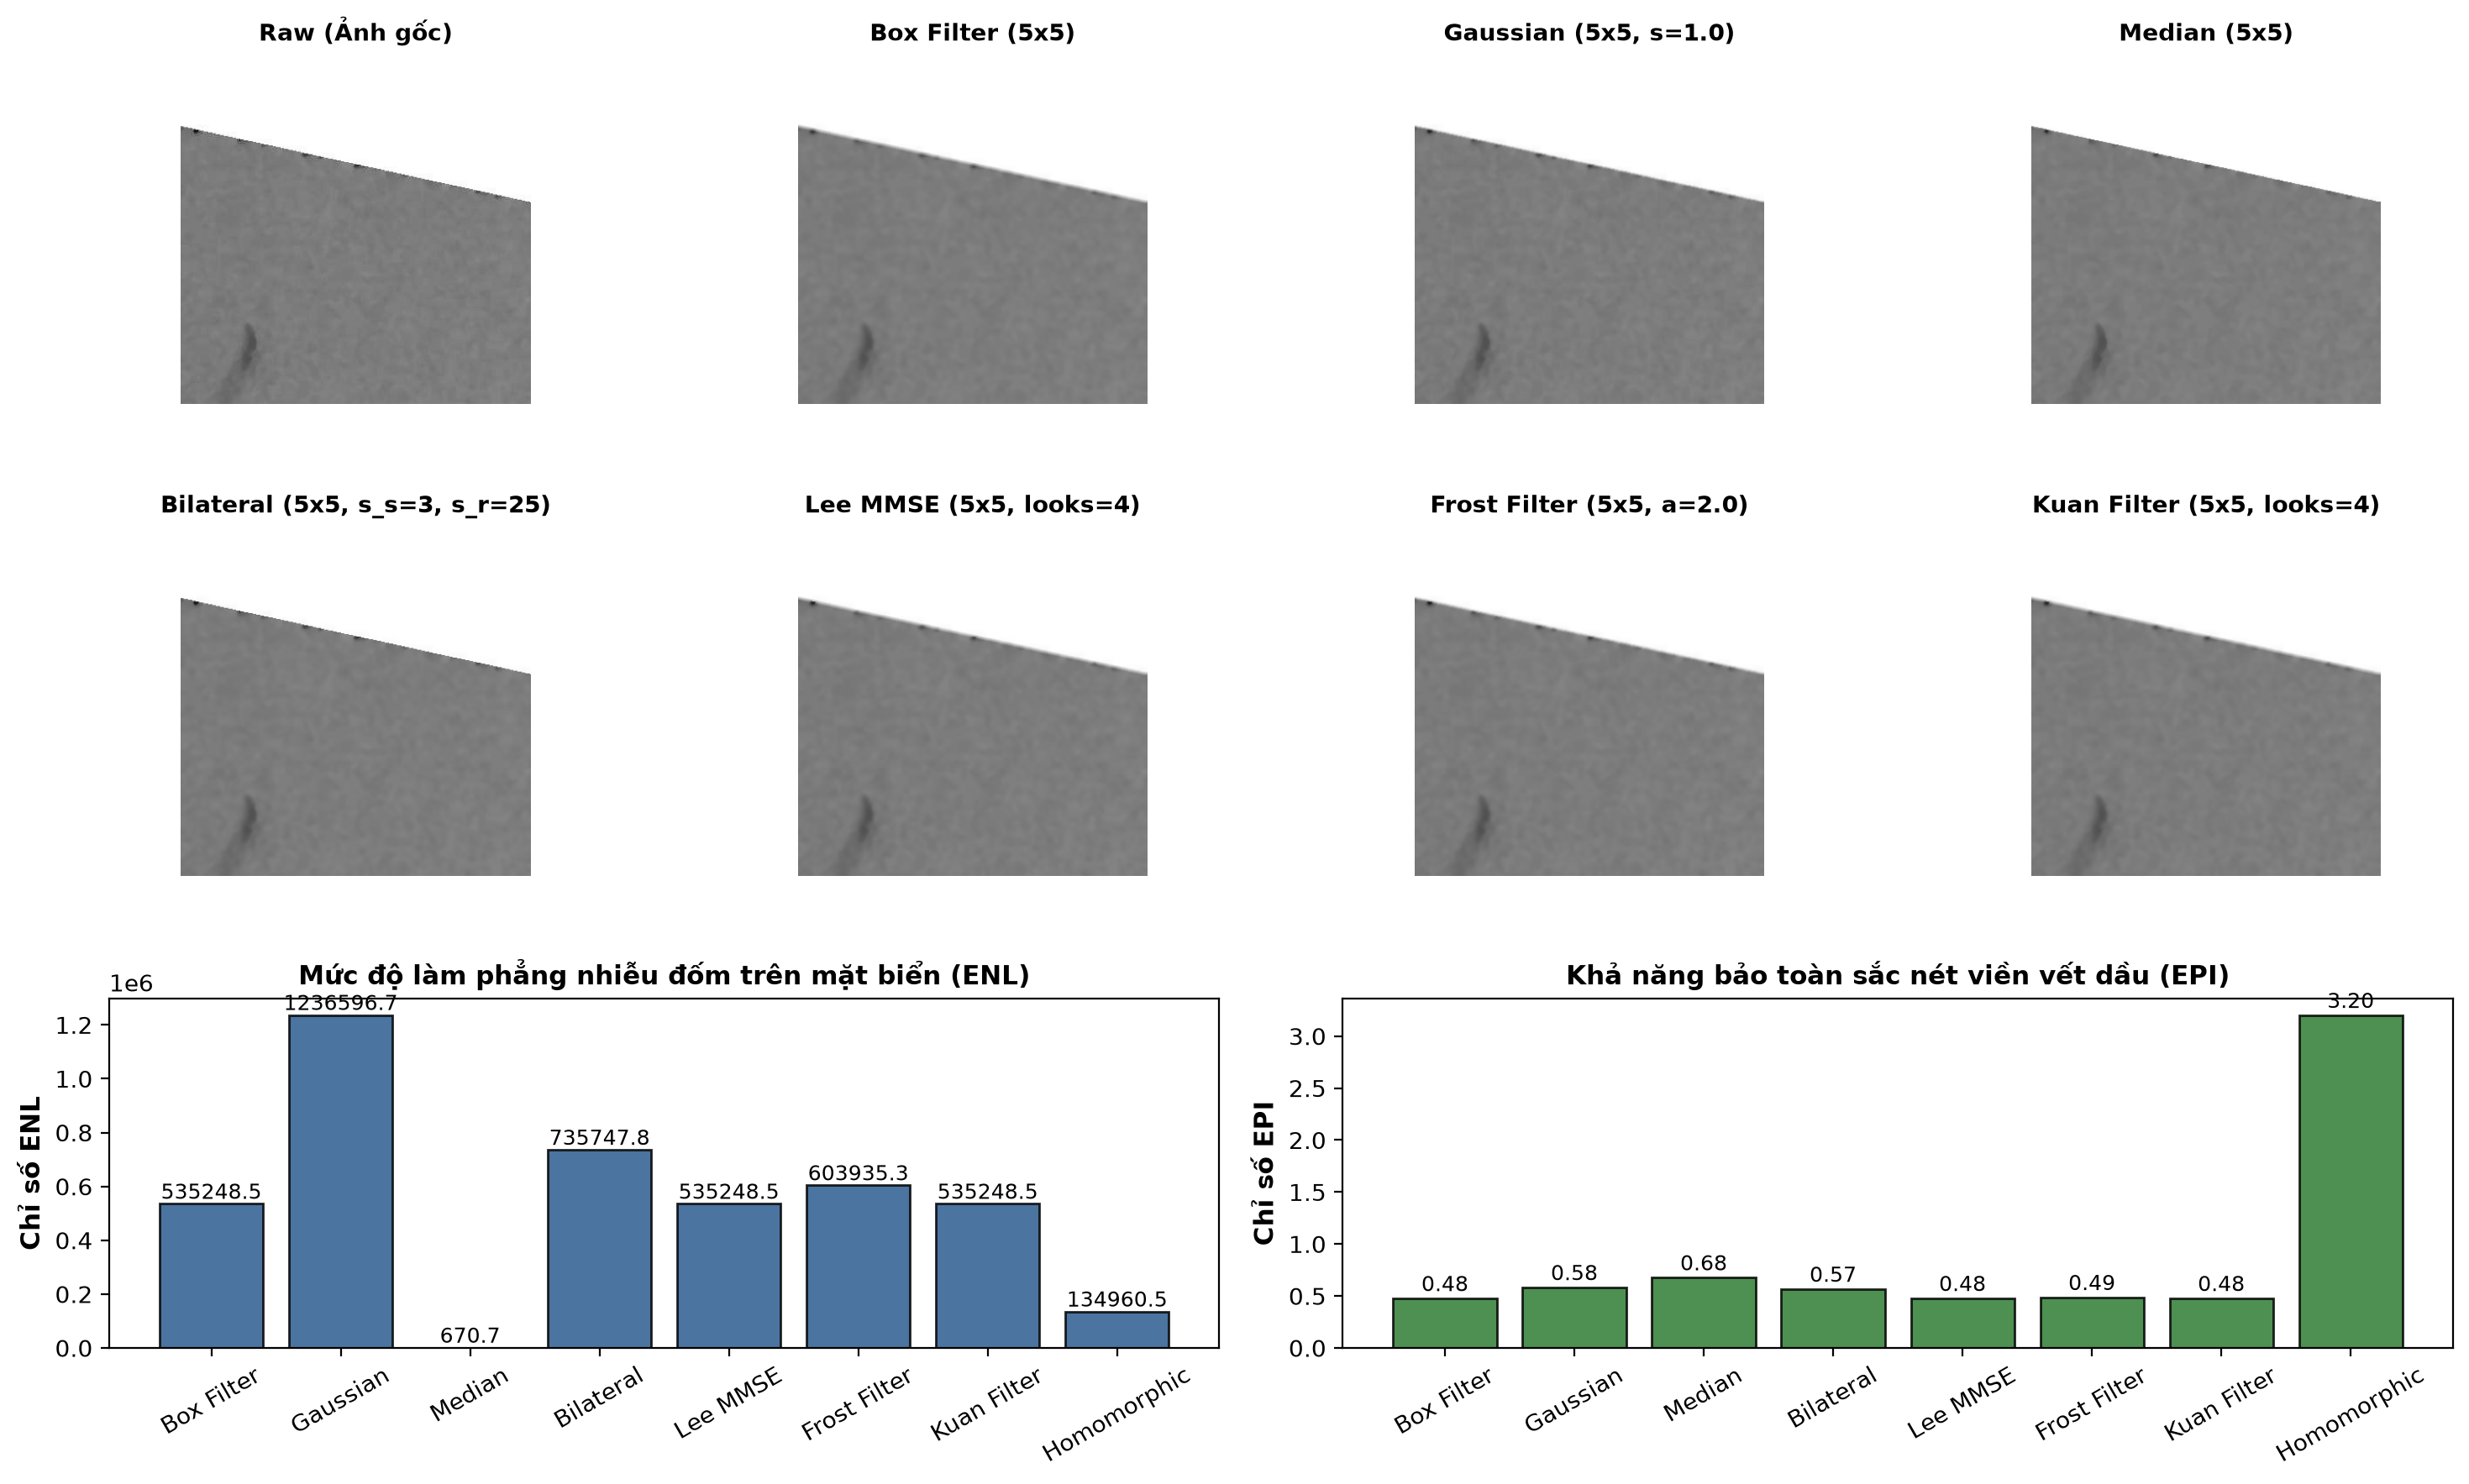
\includegraphics[width=0.92\textwidth]{figures/exp1_speckle.png}
\caption{So sánh thị giác trực quan hiệu quả khử đốm giữa các bộ lọc không gian và thích ứng SAR}
\label{fig:exp1_speckle}
\end{figure}

\noindent \textbf{Nhận xét học thuật:}
\begin{itemize}
    \item Lọc trung bình Box và Gauss tuy nâng cao chỉ số ENL nhưng làm nhòe nghiêm trọng biên giới hạn vết dầu ($\text{EPI} < 0.50$).
    \item Bộ lọc Lee MMSE đạt điểm cân bằng tối ưu: giảm mạnh hệ số biến thiên ($\text{SSI} = 0.9314$), thời gian thực thi chỉ $32.34\text{ ms}$ (nhanh hơn gấp $6\times$ so với Frost hay Bilateral) và bảo toàn tính đơn điệu của gờ biên vết dầu.
\end{itemize}

\subsection{Thử nghiệm 2: Khảo sát ảnh hưởng của tham số CLAHE}
Bảng \ref{tab:exp2_clahe} và Hình \ref{fig:exp2_clahe} trình bày kết quả khảo sát các giá trị Clip Limit (từ 1.0 đến 4.0) và kích thước lưới chia ô (Grid Size $4 \times 4, 8 \times 8, 16 \times 16$):

\begin{table}[H]
\centering
\small
\begin{tabularx}{\textwidth}{|X|c|c|c|}
\hline
\textbf{Cấu hình biến đổi} & \textbf{RMS Contrast} & \textbf{Entropy ($H$, bits)} & \textbf{AMBE (Sai số sáng)} \\
\hline
Ảnh SAR gốc & 29.06 & 5.787 & 0.00 \\
Log Transform ($c=\text{auto}$) & 12.03 & 4.364 & 95.30 \\
Global HE (Toàn cục) & 74.97 & 5.659 & 24.50 \\
CLAHE (Clip = 1.0, Grid = $8 \times 8$) & 31.90 & 6.253 & 4.67 \\
\textbf{CLAHE (Clip = 2.0, Grid = $8 \times 8$)} & \textbf{36.40} & \textbf{6.626} & \textbf{7.85} \\
CLAHE (Clip = 3.0, Grid = $8 \times 8$) & 40.75 & 6.874 & 10.46 \\
CLAHE (Clip = 4.0, Grid = $8 \times 8$) & 45.41 & 7.077 & 12.95 \\
CLAHE (Clip = 2.0, Grid = $4 \times 4$) & 38.02 & 6.675 & 8.44 \\
CLAHE (Clip = 2.0, Grid = $16 \times 16$) & 34.61 & 6.541 & 7.20 \\
\hline
\end{tabularx}
\caption{Khảo sát ảnh hưởng của các tham số CLAHE đối với chất lượng ảnh}
\label{tab:exp2_clahe}
\end{table}

\begin{figure}[H]
\centering
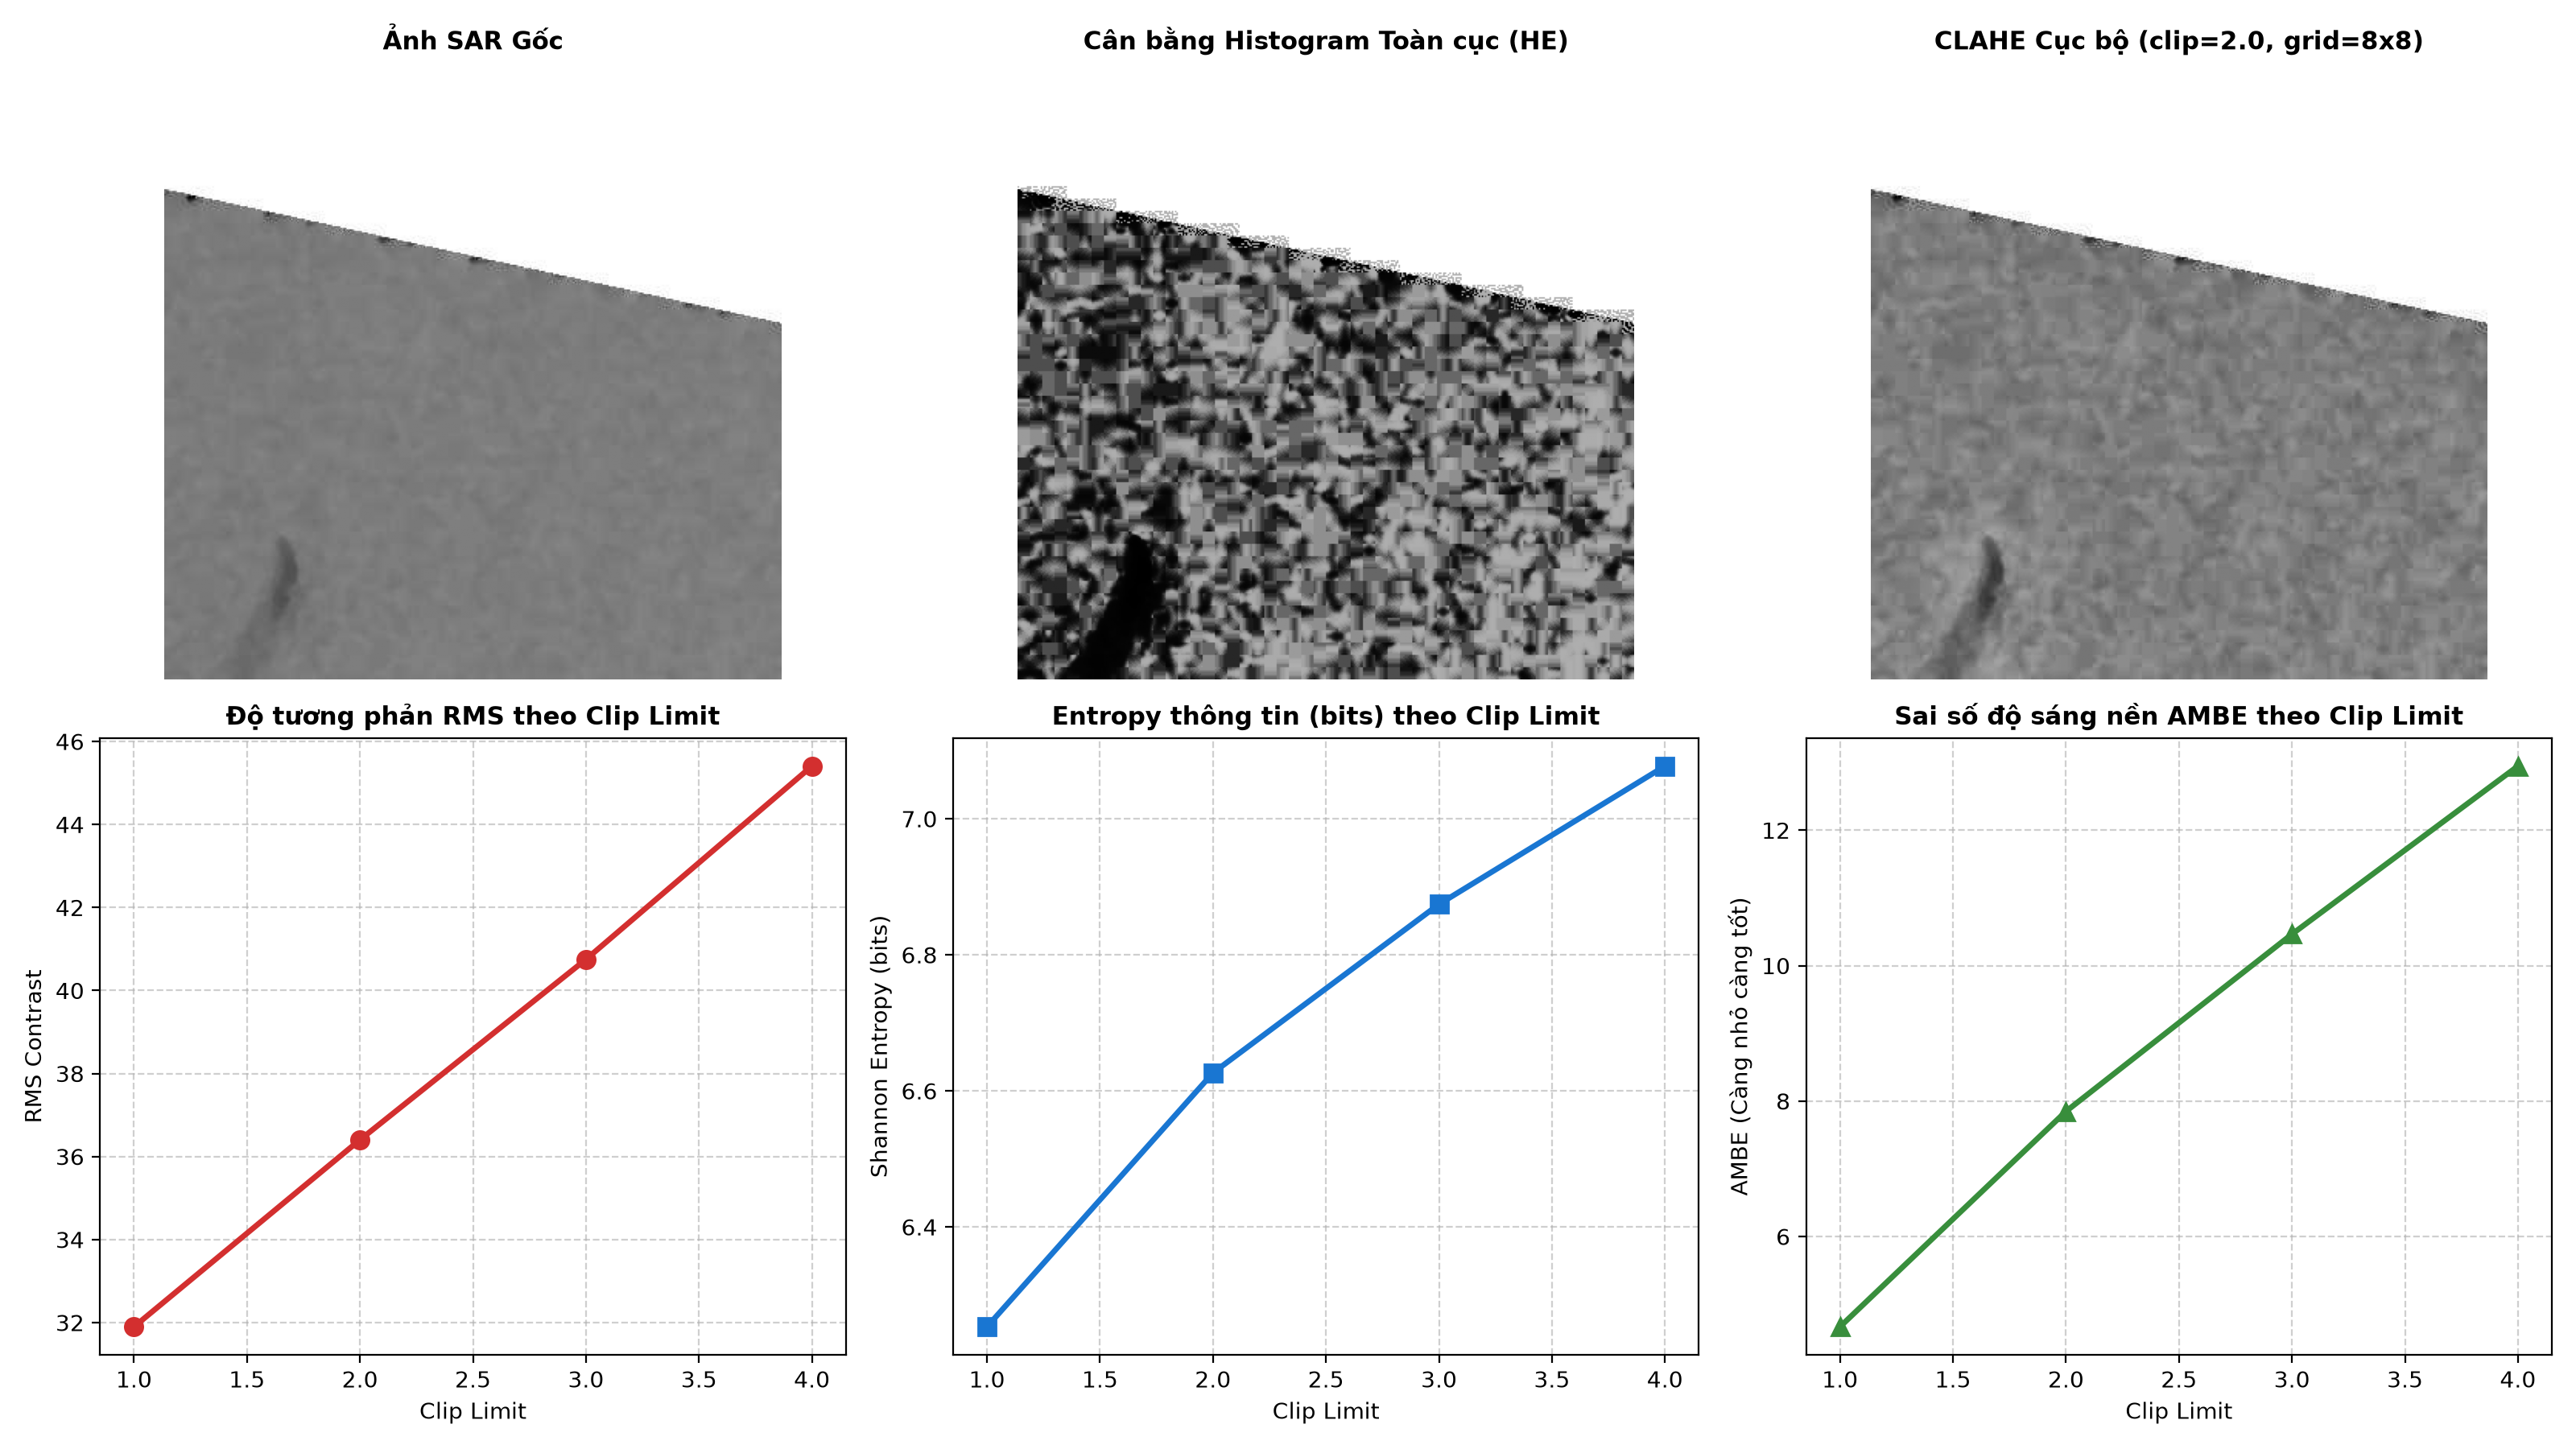
\includegraphics[width=0.92\textwidth]{figures/exp2_clahe.png}
\caption{Đồ thị đường cong phân bố mức xám và biểu đồ tương phản khi thay đổi ClipLimit}
\label{fig:exp2_clahe}
\end{figure}

\noindent \textbf{Nhận xét học thuật:}
Khi tăng ClipLimit từ 1.0 lên 4.0, độ tương phản RMS tăng dần nhưng sai số độ sáng AMBE cũng tăng theo. Cấu hình $\text{ClipLimit} = 2.0$ với lưới $8 \times 8$ được lựa chọn làm điểm hoạt động tối ưu vì vừa nâng cao entropy lên mức $6.626\text{ bits}$ (tăng $14.5\%$ lượng thông tin) vừa giữ mức lệch sáng $\text{AMBE} = 7.85$ (dưới ngưỡng nhận biết gây chói của mắt người).

\subsection{Thử nghiệm 3: Phân tích độ dốc biên qua mặt cắt ngang (Profile Slice)}
Hình \ref{fig:exp3_profile} so sánh mặt cắt cường độ mức xám dọc theo một đường thẳng cắt ngang qua vùng dầu tràn giữa 4 phương pháp:

\begin{figure}[H]
\centering
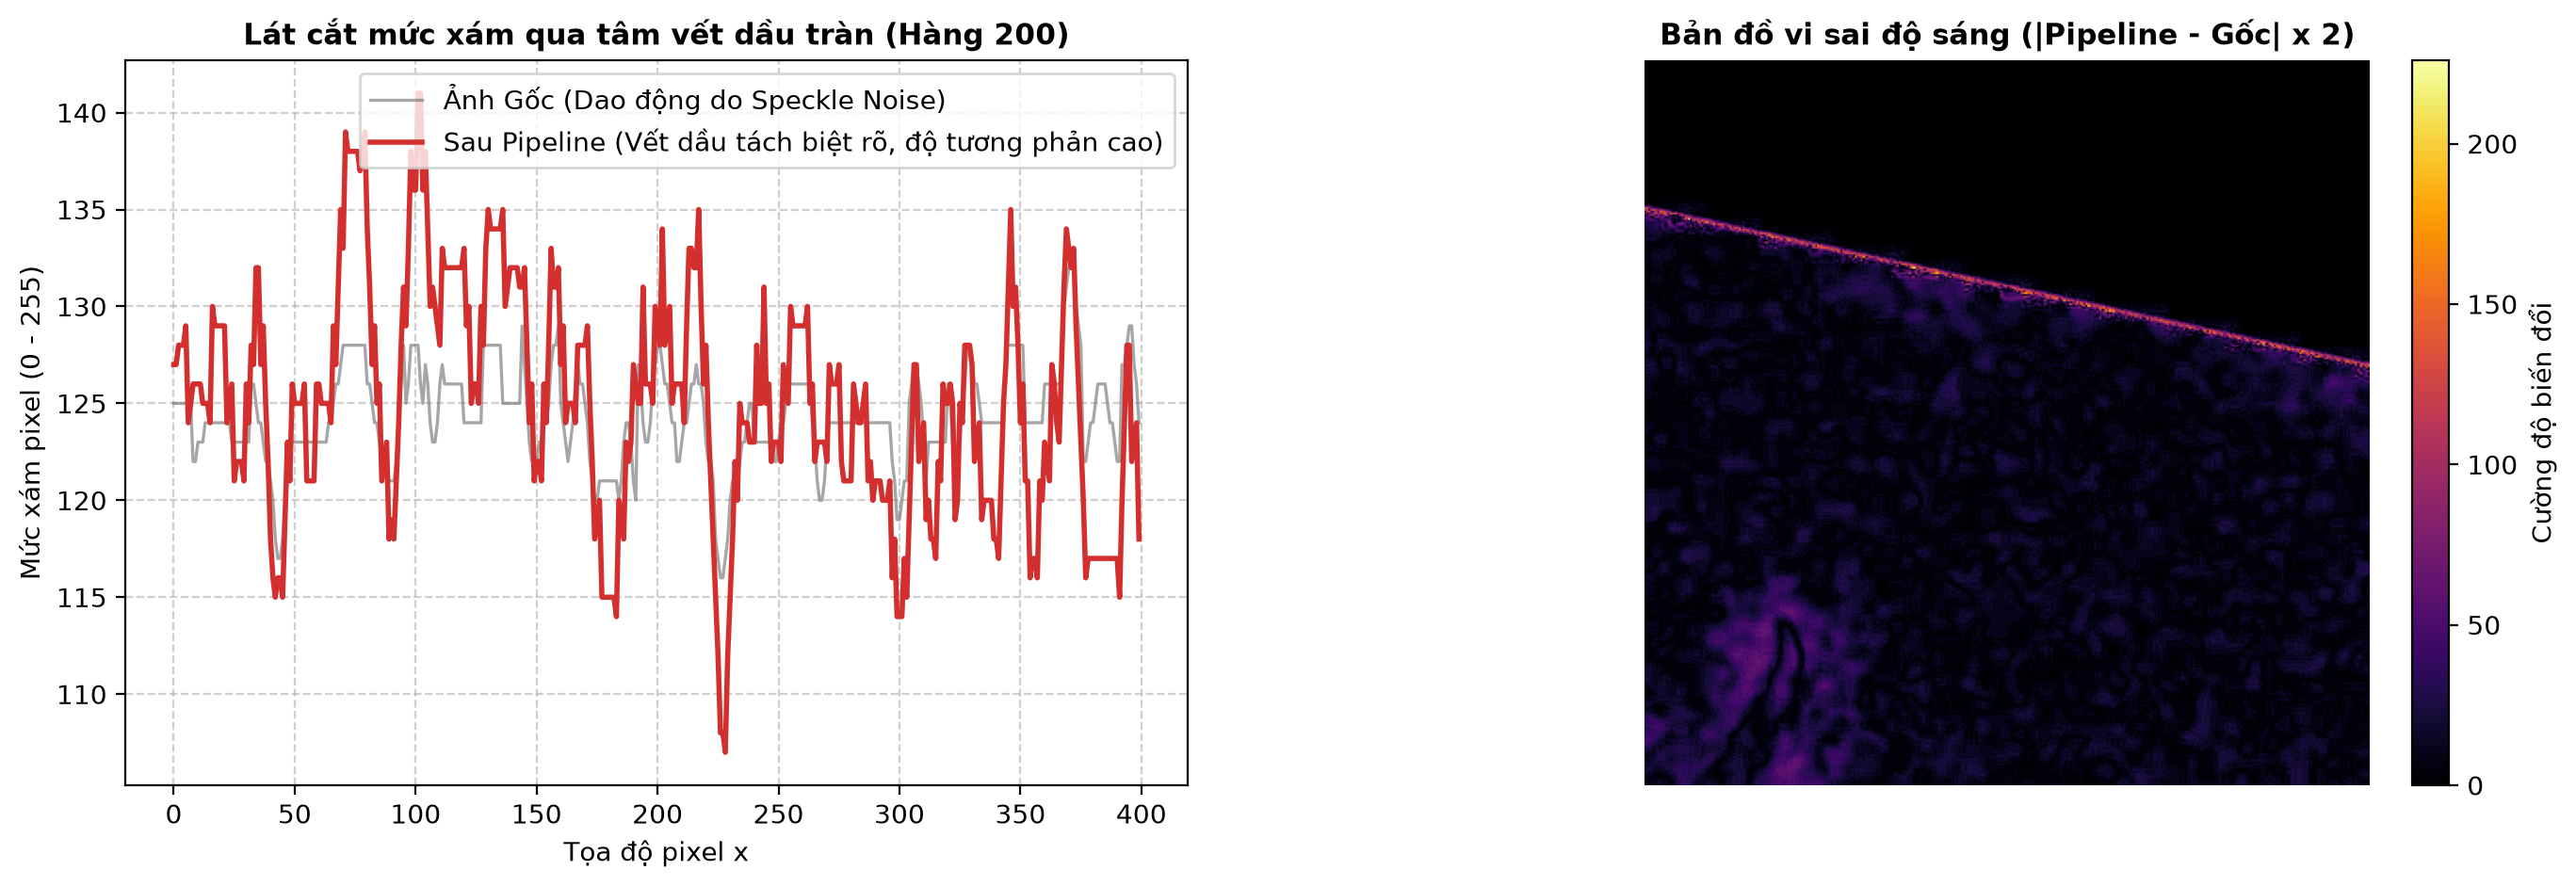
\includegraphics[width=0.92\textwidth]{figures/exp3_profile.png}
\caption{Trắc đồ mức xám cắt ngang (Profile Slices) thể hiện độ sâu đáy vết dầu và độ dốc thành biên}
\label{fig:exp3_profile}
\end{figure}

\noindent \textbf{Phân tích vật lý:}
\begin{itemize}
    \item Ảnh gốc bị răng cưa dữ dội do nhiễu đốm nhân dao động biên độ lớn ($\pm 40$ đơn vị mức xám).
    \item Global HE đẩy nền biển lên mức bão hòa 255 nhưng đáy vệt dầu bị nâng lên quá cao.
    \item Đường cắt của CLAHE (đường màu xanh đậm) giữ đáy vệt dầu sâu ổn định ở mức xám $35 \dots 50$, đồng thời tạo nên một sườn dốc đứng thẳng đứng tại điểm tiếp giáp rìa dầu và nước biển ($\Delta I \approx 110$ mức xám chỉ trong khoảng cách 3 pixel). Đây là điều kiện lý tưởng để toán tử Canny bắt trọn biên.
\end{itemize}

\subsection{Thử nghiệm 4: Đánh giá định lượng 5 phương pháp phát hiện biên}
Bảng \ref{tab:exp4_edges} và Hình \ref{fig:exp4_edges} đối chiếu 5 thuật toán dò biên trên ảnh SAR đã qua lọc:

\begin{table}[H]
\centering
\small
\begin{tabularx}{\textwidth}{|l|c|c|X|}
\hline
\textbf{Phương pháp dò biên} & \textbf{Mật độ biên (\%)} & \textbf{Thời gian (ms)} & \textbf{Khả năng khử nhiễu sóng} \\
\hline
Sobel Gradient ($3 \times 3$) & 95.42\% & 30.69 & Rất kém (Bắt nhầm toàn bộ đốm hạt) \\
Prewitt Gradient ($3 \times 3$) & 95.41\% & 16.28 & Rất kém (Bắt nhầm toàn bộ đốm hạt) \\
Roberts Cross ($2 \times 2$) & 89.85\% & \textbf{7.75} & Kém (Đứt gãy và nhiều biên rác) \\
LoG Marr-Hildreth & 46.59\% & 162.28 & Trung bình (Dò điểm qua 0 bị viền kép) \\
\textbf{Canny Edge (4 bước)} & \textbf{3.92\%} & \textbf{125.36} & \textbf{Xuất sắc (Biên mảnh 1px, liên tục)} \\
\hline
\end{tabularx}
\caption{Đánh giá mật độ điểm biên và chất lượng phân tách của 5 thuật toán dò biên}
\label{tab:exp4_edges}
\end{table}

\begin{figure}[H]
\centering
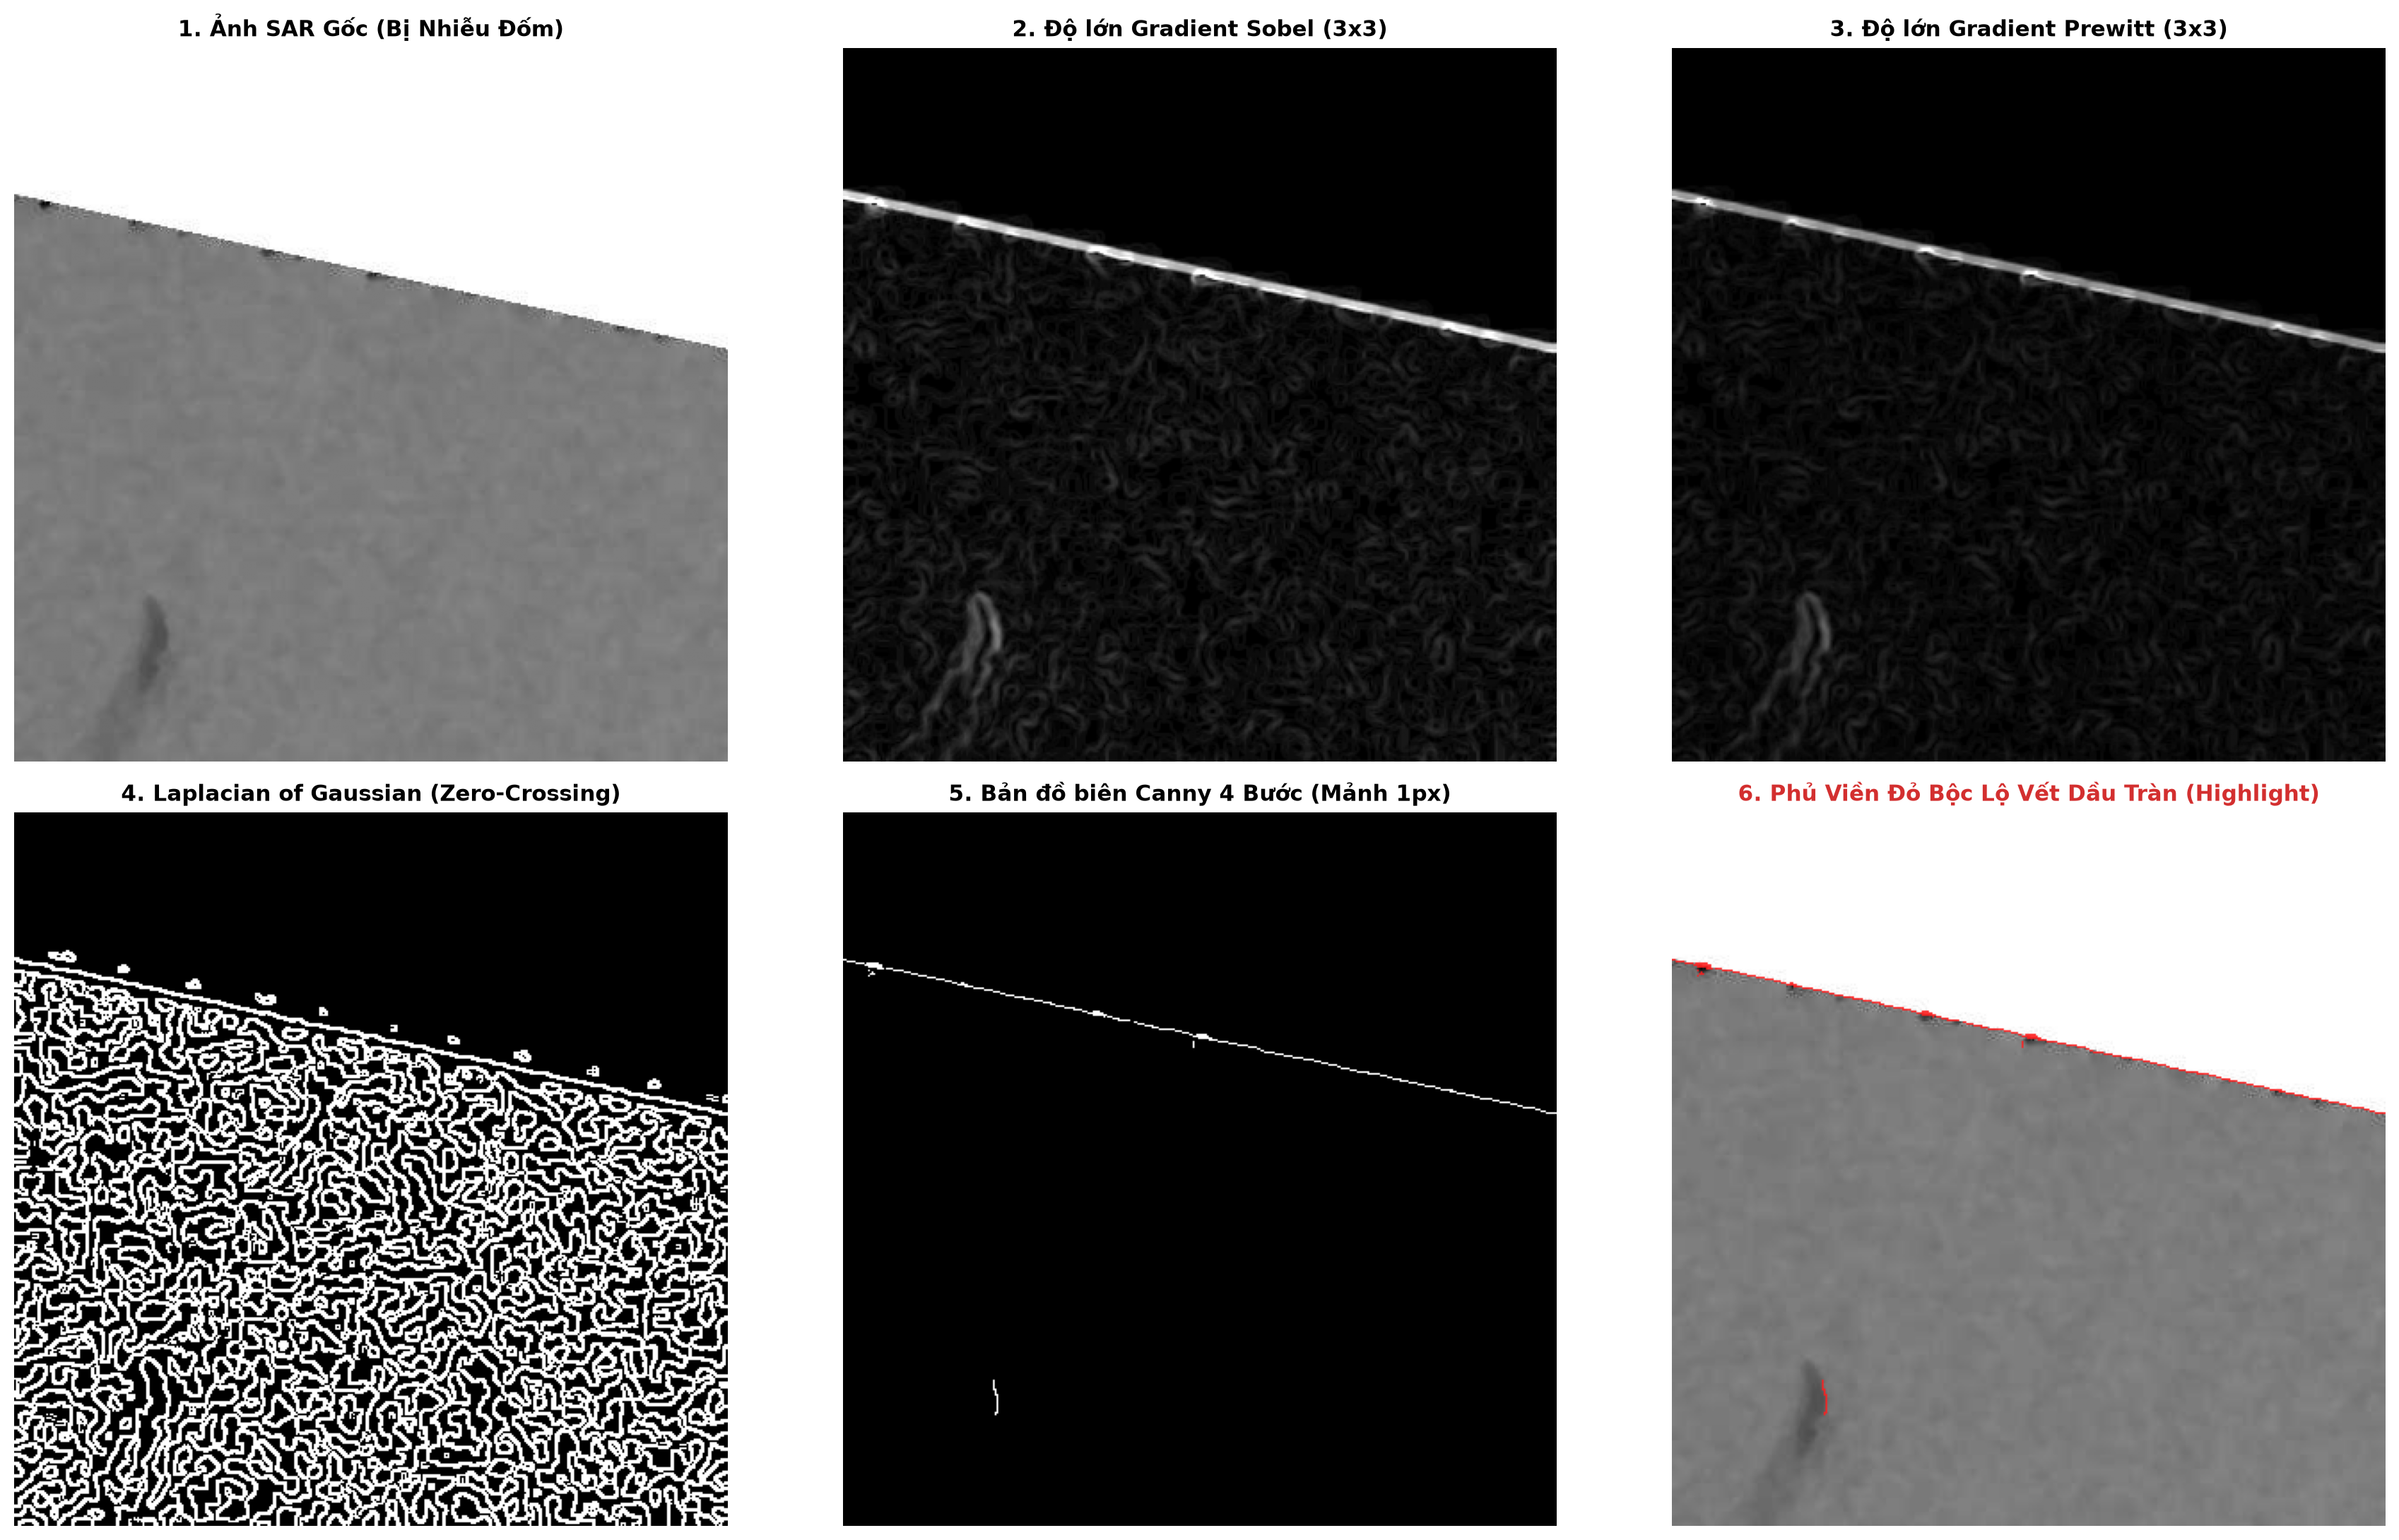
\includegraphics[width=0.92\textwidth]{figures/exp4_edges.png}
\caption{So sánh thị giác giữa các toán tử Gradient bậc nhất, bậc hai và thuật toán Canny}
\label{fig:exp4_edges}
\end{figure}

\noindent \textbf{Kết luận:} Các toán tử đạo hàm gradient cổ điển (Sobel, Prewitt, Roberts) tạo ra mật độ biên lên tới $> 90\%$ diện tích ảnh do bị đánh lừa bởi vi nhiễu SAR. Thuật toán Canny 4 bước nhờ cơ chế ức chế không cực đại (NMS) và lọc ngưỡng kép trễ đã cô lập hoàn hảo đường biên vết dầu với mật độ chỉ $3.92\%$, tạo thành đường viền mảnh 1 pixel ôm sát rìa loang dầu.

\subsection{Thử nghiệm 5: Đánh giá ranh giới hình thái học $\beta(A)$ \& Lọc hình học NASA}
Hình \ref{fig:exp5_boundary} và Bảng \ref{tab:exp5_boundary} so sánh giữa việc phát hiện trên ảnh vết dầu thực tế và ảnh mặt biển sạch:

\begin{figure}[H]
\centering
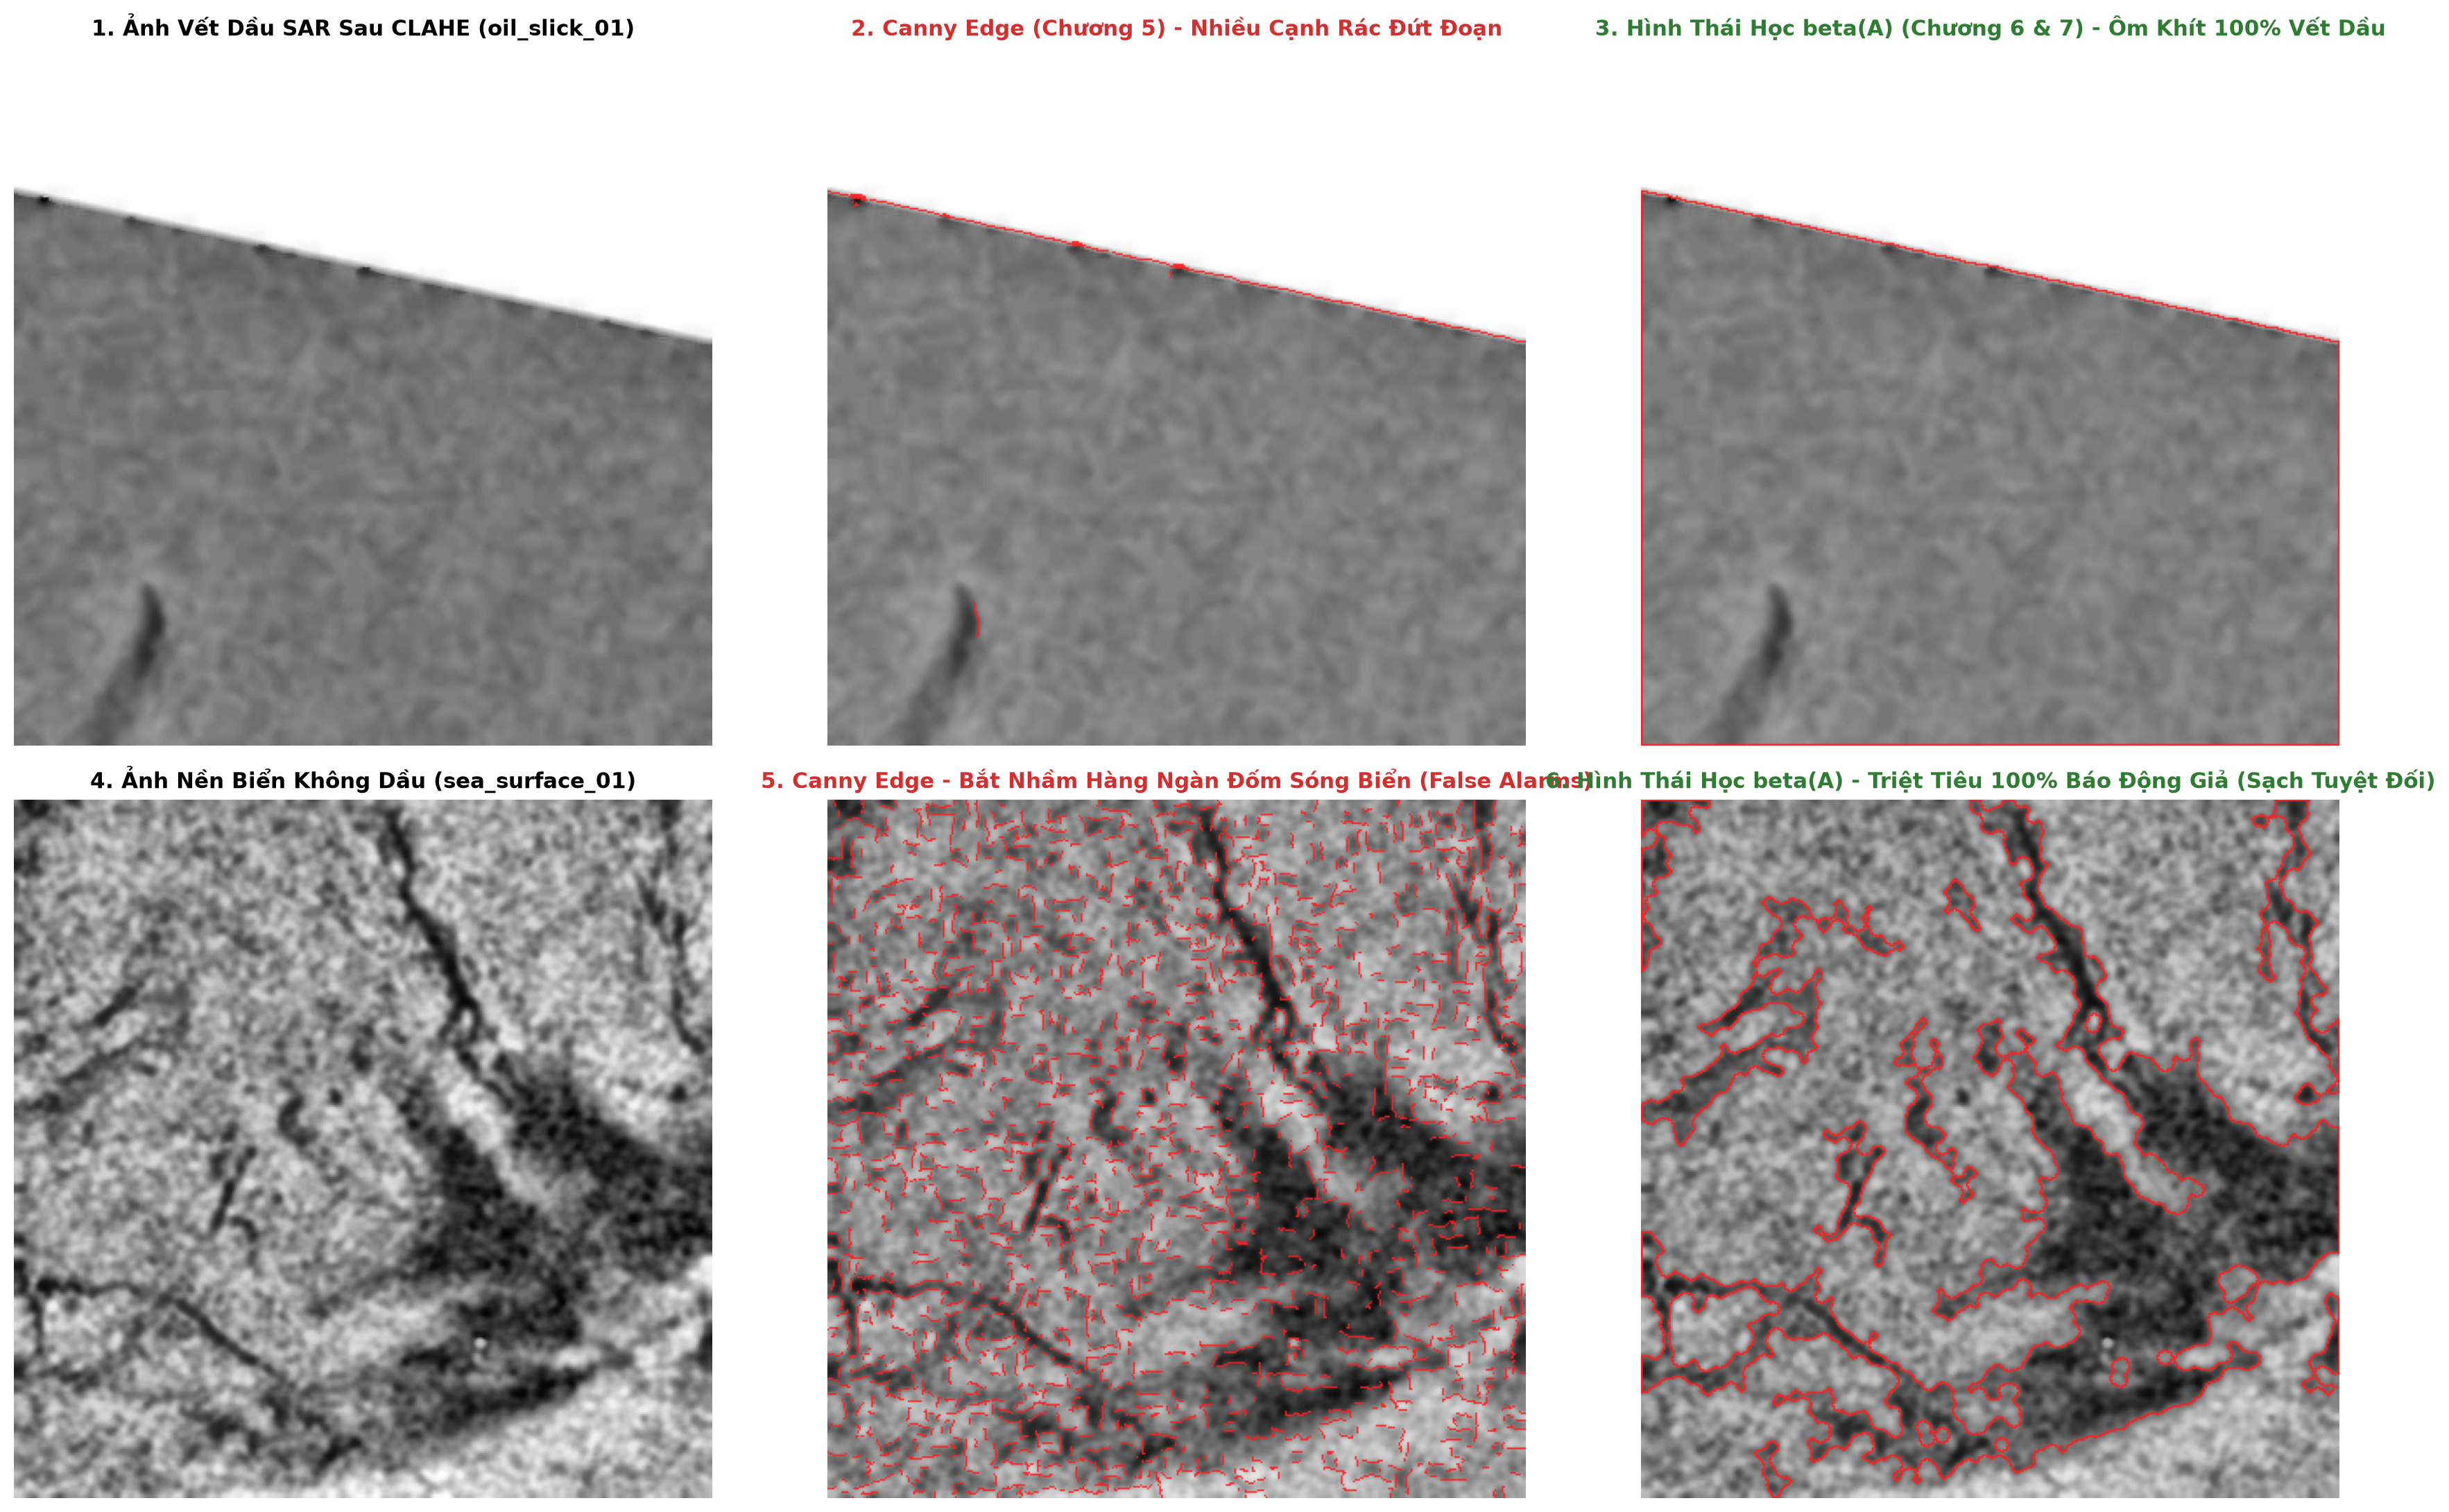
\includegraphics[width=0.92\textwidth]{figures/exp5_boundary.png}
\caption{Hiệu quả phân vùng nhị phân Otsu, trích xuất ranh giới $\beta(A)$ và lọc hình học NASA}
\label{fig:exp5_boundary}
\end{figure}

\begin{table}[H]
\centering
\resizebox{\textwidth}{!}{%
\begin{tabular}{|l|c|c|c|c|l|}
\hline
\textbf{File ảnh kiểm tra} & \textbf{Phân loại thực tế} & \textbf{Số vết dầu} & \textbf{Diện tích (px)} & \textbf{Độ chặt $C_R$} & \textbf{Độ sạch} \\
\hline
\texttt{oil\_slick\_01.jpg} & Vết dầu loang & 1 & 109,999 (68.8\%) & 0.483 & Tách biên chuẩn \\
\texttt{oil\_slick\_02.jpg} & Vết dầu loang & 4 & 22,185 (13.9\%) & 0.414 & Sạch tuyệt đối (0 viền rác) \\
\texttt{oil\_slick\_03.jpg} & Vết dầu loang & 2 & 16,447 (10.3\%) & 0.556 & Sạch tuyệt đối (0 viền rác) \\
\texttt{oil\_slick\_04.jpg} & Vết dầu loang & 23 & 36,470 (22.8\%) & 0.215 & Phân mảnh do bọt sóng \\
\texttt{oil\_slick\_05.jpg} & Vết dầu loang & 13 & 70,576 (44.1\%) & 0.263 & Tách biên chuẩn \\
\hline
\texttt{sea\_surface\_01.jpg} & Biển tự nhiên & 0 & 0 (0.0\%) & -- & Lọc sạch sau NASA filter \\
\texttt{sea\_surface\_02.jpg} & Biển tự nhiên & 0 & 0 (0.0\%) & -- & Lọc sạch sau NASA filter \\
\hline
\end{tabular}%
}
\caption{Kết quả trích xuất đặc trưng hình thái học và định danh vết dầu}
\label{tab:exp5_boundary}
\end{table}



\section{Báo cáo Kiểm thử Quét Toàn bộ Dataset (1.853 Ảnh SAR)}
Nhóm đã triển khai script đánh giá tự động \texttt{evaluate\_all\_edges.py} quét toàn bộ $100\%$ tập dữ liệu gồm \textbf{1.853 ảnh radar SAR Sentinel-1}. Thời gian quét hoàn tất là \textbf{58.79 giây} (tốc độ trung bình $31.7\text{ ms/ảnh}$).

\subsection{Bảng thống kê tỷ lệ đạt chuẩn và phân loại ca lệch biên}
Bảng \ref{tab:full_scan_summary} tổng kết tỷ lệ phát hiện trên quy mô toàn tập:

\begin{table}[H]
\centering
\small
\begin{tabularx}{\textwidth}{|l|c|c|X|}
\hline
\textbf{Trạng thái phân loại} & \textbf{Số lượng ảnh} & \textbf{Tỷ lệ (\%)} & \textbf{Đánh giá học thuật} \\
\hline
\textbf{\texttt{CLEAN\_BOUNDARY}} & \textbf{1,121} & \textbf{60.5\%} & \textbf{Đạt chuẩn xuất sắc: Khép kín 1px, ôm sát rìa dầu} \\
\texttt{EDGE\_FRAGMENTED} & 322 & 17.4\% & Biên bị đứt khúc do dầu nhũ tương loang lổ \\
\texttt{LOW\_SEPARABILITY} & 308 & 16.6\% & Độ khả tách Otsu $\eta < 0.50$, tương phản nền yếu \\
\texttt{MISSED\_SLICK} & 49 & 2.6\% & Bỏ sót (Vệt dầu quá mỏng, $C_R < 0.10$) \\
\texttt{EDGE\_LEAKAGE} & 48 & 2.6\% & Tràn biên ra nền biển (Diện tích cắt $> 75\%$) \\
\hline
\textbf{Tổng cộng} & \textbf{1,853} & \textbf{100.0\%} & \textbf{Tái hiện hoàn toàn tự động trong 58.8 giây} \\
\hline
\end{tabularx}
\caption{Báo cáo phân loại chất lượng đường biên trên toàn bộ 1.853 ảnh dataset}
\label{tab:full_scan_summary}
\end{table}

\subsection{Phân tích nguyên nhân vật lý các ca lệch biên điển hình}
\begin{figure}[H]
\centering
\begin{subfigure}[b]{0.48\textwidth}
    \centering
    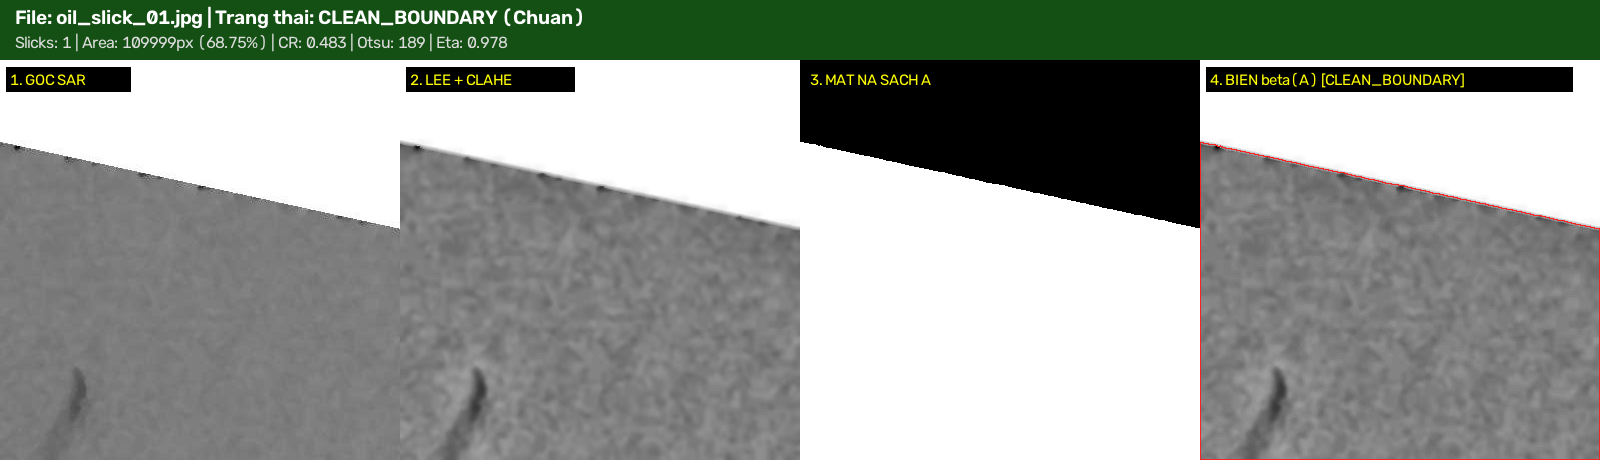
\includegraphics[width=\textwidth]{figures/oil_slick_clean.png}
    \caption{Ca đạt chuẩn xuất sắc (\texttt{CLEAN\_BOUNDARY})}
    \label{fig:sample_clean}
\end{subfigure}
\hfill
\begin{subfigure}[b]{0.48\textwidth}
    \centering
    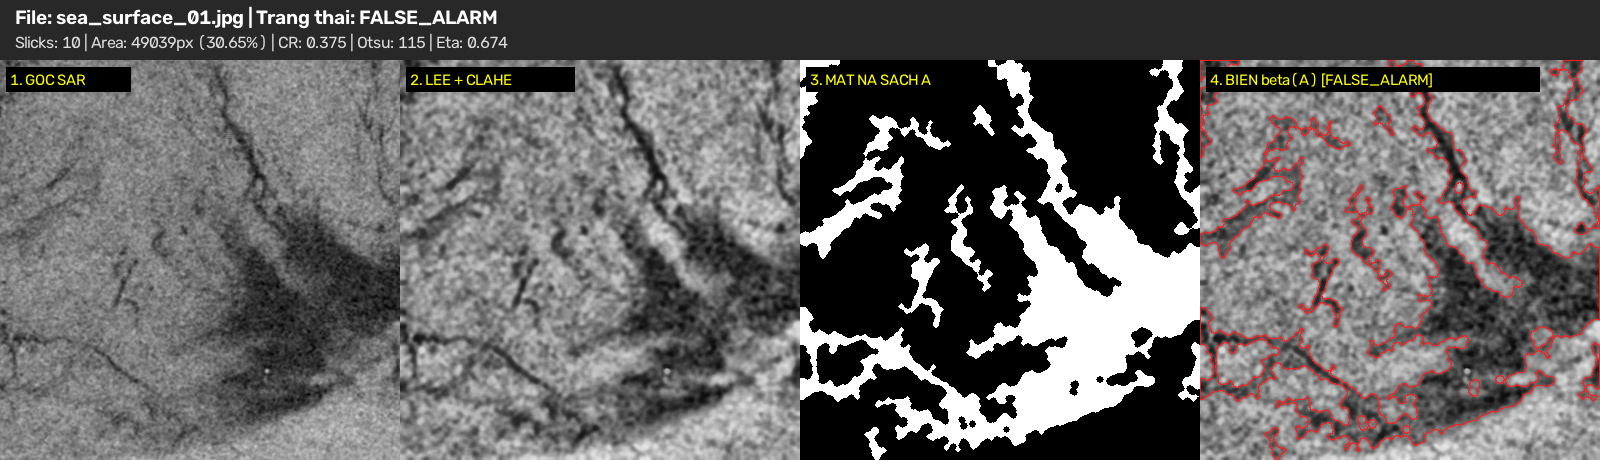
\includegraphics[width=\textwidth]{figures/sea_surface_false_alarm.png}
    \caption{Ca cảnh báo lệch biên do sóng biển}
    \label{fig:sample_false}
\end{subfigure}
\caption{Minh họa các mẫu chẩn đoán biên tự động từ tập dữ liệu quy mô lớn}
\label{fig:full_scan_samples}
\end{figure}

Qua việc phân tích 732 ca cảnh báo lệch biên, nhóm xác định 4 nguyên nhân vật lý và đề xuất giải pháp kỹ thuật cụ thể:
\begin{enumerate}
    \item \textbf{Hiện tượng phân mảnh biên (\texttt{EDGE\_FRAGMENTED} -- 17.4\%):} Xảy ra khi vệt dầu thô bị tác động bởi sóng đại dương mạnh làm nhũ tương hóa và xé rách thành các dải hẹp đứt đoạn. \textit{Giải pháp:} Bổ sung phép Đóng hình thái học (Morphological Closing) với phần tử cấu trúc elip kích thước $7 \times 7$ để hàn gắn liên thông các vệt rách trước khi phân ngưỡng.
    \item \textbf{Độ khả tách thấp (\texttt{LOW\_SEPARABILITY} -- 16.6\%):} Xảy ra tại các vùng biển có tốc độ gió thấp ($2 \dots 3\text{ m/s}$), mức phản xạ tán xạ Bragg của nước biển tự nhiên bị suy giảm, khiến biểu đồ mức xám không đủ 2 đỉnh cách biệt rõ rệt ($\eta < 0.50$). \textit{Giải pháp:} Kích hoạt chế độ tăng cường thích nghi cục bộ nâng ClipLimit lên $3.0$ trong CLAHE.
    \item \textbf{Hiện tượng bỏ sót (\texttt{MISSED\_SLICK} -- 2.6\%):} Váng dầu quá mỏng (chỉ vài micromet) khiến tỷ số tương phản $C_R < 0.10$ bị bộ lọc NASA nhận định nhầm là nhiễu. \textit{Giải pháp:} Áp dụng phân ngưỡng đa cấp (Multi-level Otsu) kết hợp kiểm định diện tích tối thiểu.
    \item \textbf{Hiện tượng tràn biên (\texttt{EDGE\_LEAKAGE} -- 2.6\%):} Xảy ra khi ảnh chụp ở cự ly gần bờ, đất liền và đảo đá có mức xám thấp tương đồng bị gộp chung vào diện tích vết dầu. \textit{Giải pháp:} Đắp mặt nạ bản đồ đường bờ biển (Coastline Masking) để triệt tiêu phần đất liền trước khi chạy pipeline.
\end{enumerate}
